\section{Background and Problem Setup}\label{background}
This section describes the challenges in predictive modeling after progressive data 
cleaning and describes concrete example applications.

\subsection{Machine Learning and Data Cleaning}\label{alrw}
Machine learning can be used as a technique to improve the efficiency and/or reliability of data cleaning\cite{yakout2013don,gokhale2014corleone}.
For example, Yakout et al. train a statistical model that evaluates the likelihood of a proposed replacement value \cite{yakout2013don}.
Another application of machine learning is value imputation, where a missing value is predicted based on those records without missing values.
Machine learning is also increasingly applied to make automated repairs more reliable with human validation \cite{DBLP:journals/pvldb/YakoutENOI11}.
Human input is often expensive and impractical to apply to entire large datasets.
Machine learning can extrapolate rules from a small set of examples cleaned by a human (or humans) to uncleaned data \cite{gokhale2014corleone, DBLP:journals/pvldb/YakoutENOI11}.
This approach can be coupled with active learning \cite{DBLP:journals/pvldb/MozafariSFJM14} to learn an accurate model with the fewest possible number of examples, and intuitively, this means
query a human only when the statistical model indicates uncertainty.

A common thread in these approaches is a Data Cleaning Model (DCM) that learns to predict the value of an incorrect or missing attribute given data that are previously cleaned or known to be clean.
In contrast, \sys addresses the problem of statistical analysis, in the form of Machine Learning, on clean data.
We call such models Downstream Statistical Models (DSMs) to contrast them with the DCMs in prior work.
An example of a DSM is a movie recommender system that collects dirty user preference data resulting in error-prone predictions.
The DSM is independent of the errors manifest in the data and is specified by the user.
The DSM problem is more general than the DCM problem with a broader class of allowed statistical models, that is not just record value-prediction for data cleaning operations.
For example, a ``label" in a DSM may be a function of multiple dirty and clean attributes.
There are two key challenges in applying data cleaning before a DSM: (1) statistical validity, and (2) efficiency. 
\sys addresses both of these challenges using an incremental update framework that ensures correctness of intermediate results and several novel extensions to active learning, including dirty data detection and estimation, to clean data that maximally benefit a DSM.

It turns out that our method for model update and active learning with DSMs includes many types of DCMs.
Consider the deduplication problem with active learning as studied in Gokhale et al. \cite{gokhale2014corleone}.
In this problem, humans label pairs of records as entity matches or not.
We could create a relation $R \times R$ with all pairs of records and an extra missing attribute corresponding to the label. 
Our DSM could be a classifier that predicts whether the pair is a match or not.
All of the optimizations in \sys would apply, however, it is likely that Gokhale et al. would be more efficient exploiting problem specific structure such as transitivity.

\subsection{Dirty Data Model}\label{dmodel}
\sys supports data cleaning algorithms that can be represented as record-by-record transformations.
Formally, there exists a function (implemented via human or algorithm) that when given a dirty record, it will return a unique clean record.
This does not cover errors that simultaneously affect multiple records such as record duplication or schema transformation problems.
We represent this operation as $C(\cdot)$ which can be applied to a record $r$ to recover $r_{clean} = C(r)$.
Therefore, for every $r \in R_{dirty}$ there exists a unique $r' \in R_{clean}$.
We assume that there is a featurization $F(\cdot)$ which is defined over both $R_{dirty}$ and $R_{clean}$ and maps records to tuple of vectors in $(\mathbb{R}^d, \mathbb{R}^l)$ corresponding to features and labels.
So each record corresponds to one training example in the downstream model.

\subsection{Correctness}\label{correctness}  
%The key challenge in \sys is correctness of the statistical model.
The straight-forward application of progressive data cleaning methods is to fix those errors in place.
Suppose $k \ll N$ records are cleaned, but all of the remaining dirty records are retained in the dataset.
Figure \ref{update-arch1} highlights the dangers of this approach on a very simple dirty dataset and a linear regression model i.e., the best fit line for two variables. 
One of the variables is systematically corrupted with a translation in the x-axis (Figure \ref{update-arch1}a).
The dirty data is marked in brown and the clean data in green, and their respective best fit lines are in blue.
After cleaning only two of the data points (Figure \ref{update-arch1}b), the resulting best fit line is in the opposite direction of the true model.
This is a well-known phenomenon called Simpsons paradox, where mixtures of different populations of data can result in spurious relationships \cite{simpson1951interpretation}.
Training models on a mixture of dirty and clean data can lead to unreliable results, where artificial trends introduced by the mixture can be confused for the effects of data cleaning.

\begin{figure}[ht!]
\centering
 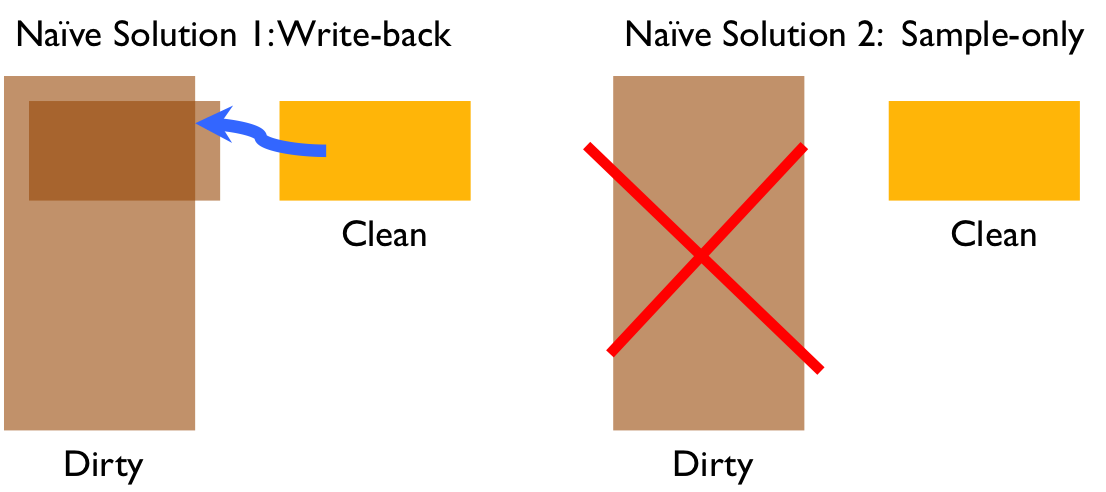
\includegraphics[width=\columnwidth]{figs/update-arch.png}
 \caption{(a) Systematic corruption in one variable can lead to a shifted model. 
 (b) Mixed dirty and clean data results in a less accurate model than no cleaning.
(c) Small samples of only clean data can result in similarly inaccurate models. \label{update-arch1}}
\end{figure}

An alternative is to avoid the dirty data altogether instead of mixing the two populations.
Suppose $k$ records are randomly sampled from the dataset and cleaned.
The model is trained only on the cleaned sample of data.
This is similar to SampleClean \cite{wang1999sample}, which was proposed to approximate the results of aggregate queries by applying them to a clean sample of data.
However, high-dimensional models are highly sensitive to sample size.
Figure \ref{update-arch1}c illustrates that, even in two dimensions, models trained from small samples can be as incorrect as the mixing solution described before.

\subsection{Intuitive Solution}
Our first goal is to find an update algorithm that avoids Simpson's Paradox and the strong dependence on sample size.
Instead of mixing dirty and clean data, \sys uses a model trained on the dirty data as an initialization, and then iteratively updates this model using samples of clean data.
The intuition is that this algorithm smoothly transitions the model from one population (the dirty data) to another (the clean data), leading to provable guarantees about intermediate results.
Our next goal is to prioritize which data to clean based on information from the model.
Doing so is not trivial since data may look unimportant to a dirty model but when cleaned are very important.
Also, data cleaning and model training can happen at very different time scales, we have to carefully budget our effort to ensure that any optimizations actually address rate-determining steps in the workflow.

\subsection{Use Case: Dollars for Docs \cite{dollarsfordocs}}\label{s:usecase}
ProPublica collected a dataset of corporate donations to doctors to analyze conflicts of interest. 
They reported that some doctors received over \$500,000 in travel, meals, and consultation expenses \cite{dollarsfordocsa}.
ProPublica laboriously curated and cleaned a dataset from the Centers for Medicare and Medicaid Services that listed nearly 250,000 research donations, and aggregated these donations by physician, drug, and pharmaceutical company.
We collected the raw unaggregated data and explored whether suspect donations could be predicted with a model.
This problem is typical of analysis scenarios based on observational data seen in finance, insurance, medicine, and investigative journalism.
The dataset has the following schema:
\begin{lstlisting}[mathescape,basicstyle={\scriptsize}]
Contribution(pi_specialty$\textrm{,}$ drug_name$\textrm{,}$ device_name$\textrm{,}$
corporation$\textrm{,}$ amount$\textrm{,}$ dispute$\textrm{,}$ status)
\end{lstlisting}

\noindent\texttt{pi\_specialty} is a textual attribute describing the specialty of the doctor receiving the donation.

\noindent\texttt{drug\_name} is the branded name of the drug in the research study (null if not a drug).

\noindent\texttt{device\_name} is the branded name of the device in the study (null if not a device).

\noindent\texttt{corporation} is the name of the pharmaceutical providing the donation.

\noindent\texttt{amount} is a numerical attribute representing the donation amount.

\noindent\texttt{dispute} is a Boolean attribute describing whether the research was disputed.

\noindent\texttt{status} is a string label describing whether the  donation was allowed under the declared research protocol. The goal is to predict disallowed  donation. 

\vspace{0.5em}

However, this dataset is very dirty, and the systematic nature of the data corruption can result in an inaccurate model.
On the ProPublica website \cite{dollarsfordocs}, they list numerous types of data problems that had to be cleaned before publishing the data (see Appendix \ref{dfd-errors}).
For example, the most significant donations were made by large companies whose names were also more often inconsistently represented in the data e.g., ``Pfizer Inc.", ``Pfizer Incorporated", ``Pfizer".
In a scenario such as this one, the effect of systematic error can be serious.
Duplicate representations could artificially reduce the correlation between these entities and suspected contributions.
There were nearly 40,000 of the 250,000 records that had either naming inconsistencies or other inconsistencies in labeling the allowed or disallowed \texttt{status}.
Without data cleaning and using a Support Vector Machine model, the detection rate of suspect donations was 66\%.
Applying the data cleaning to the entire dataset improved this rate to 97\% in the clean data (Section \ref{dfd-exp}), and the experiments describe how \sys can achieve an 80\% detection rate for less than 4000 records cleaned.


%\sys avoids both pitfalls, Simpson's paradox and sample size dependence.

\iffalse
\sys avoids both pitfalls, Simpson's paradox and sample size dependence.
In Section \ref{model-update}, we show how we do this with iterative gradient steps (i.e., incrementally moving the line based on the clean data).
This takes advantage of the dirty data as well as the clean data, but still have provable properties about the intermediate results.
The intuition is that it smoothly and iteratively transitions the model from one population (the dirty data) to another (the clean data).
In Figure \ref{sys-arch2}, we illustrate our ideal tradeoff space of sampling and data cleaning.
At two extremes we have no cleaning (just using the dirty data) and full cleaning.
%\sys is optimized for convergence for smaller sample sizes than a uniform sampling approach.

\begin{figure}[t]
\centering
 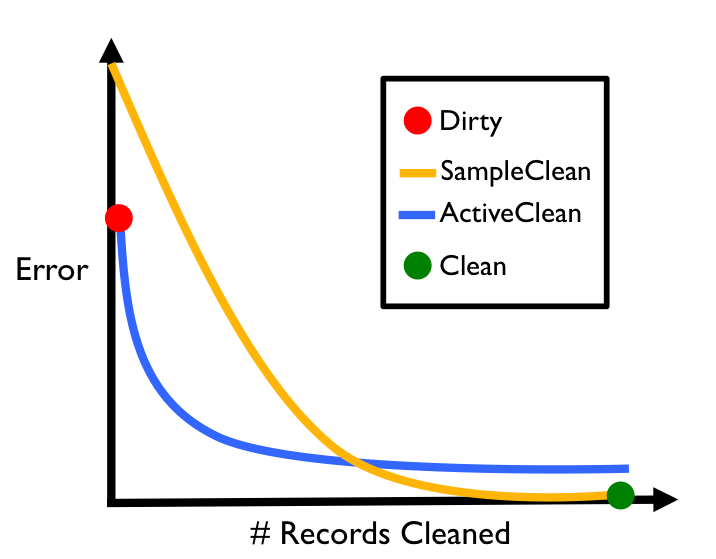
\includegraphics[width=0.5\columnwidth]{figs/arch2.png}
 \caption{\sys is designed to converge to an accurate model with fewer cleaned records than a uniform sampling approach (SampleClean). \label{sys-arch2}}\vspace{-1em}
\end{figure}


We design \sys to make greater progress at these small sample sizes using the dirty model as an initialization.
Doing so is not trivial since it requires analysis of both the Machine Learning model and the data cleaning operations.
Data may look unimportant to a dirty model but when cleaned are very important.
Also, data cleaning and model training can happen at very different time scales, we have to carefully budget our effort to ensure that any optimizations actually address rate-determining steps in the workflow.
Finally, in this line of work, the tradeoff space is enormous, and we have to carefully pick a design point and tailor our optimizations to this preferred regime.
\fi

%Consider the data corruption in our motivating example where company names were inconsistently entered: ``Pfizer Inc.", ``Pfizer Incorporated", ``Pfizer".
%Fixing this error can be represented as a record-by-record mapping.
%The data cleaning function would pick one canonical representation for the company (e.g. ``Pfizer Inc.") and map all records with other values that refer to the same real-world entity to the canonical representation.
%However, there are types of data cleaning that do not satisfy this model such as schema mapping, record deduplication, and data extractions that create additional columns. 


